\documentclass[11pt, oneside]{article}   	% use "amsart" instead of "article" for AMSLaTeX format
\usepackage{geometry}                		% See geometry.pdf to learn the layout options. There are lots.
\geometry{letterpaper}                   		% ... or a4paper or a5paper or ... 
%\geometry{landscape}                		% Activate for for rotated page geometry
%\usepackage[parfill]{parskip}    		% Activate to begin paragraphs with an empty line rather than an indent
\usepackage{graphicx}				% Use pdf, png, jpg, or eps§ with pdflatex; use eps in DVI mode
								% TeX will automatically convert eps --> pdf in pdflatex		
\usepackage{amssymb}

\title{Two Group Straight Line ANCOVA}
\author{W. Gregory Alvord} 
\date{}							% Activate to display a given date or no date

\begin{document}
\maketitle
\section{Introduction}
The simplest case of ANalysis of COVAriance (ANCOVA) is that in which there are two nominal groups and the data within each group can be fit with a straight line.  Let $ y_{ij} $ be the response for the $ i^{th} $ individual ($i = 1, ..., N) $ in the $ j^{th} $  group $(j = 1, 2) $.  Then

\begin{equation}
y_{ij} = \alpha_{j} + \beta_{j} x_{ij} + e_{ij} 
\end{equation}
where $ x_{ij} $ is the covariate for the $i^{th} $ subject ($i = 1, ..., N) $ in the $j^{th} $ group ($j = 1, 2) $ and $e_{ij} $ is the error (residual) term.  The expected value for $y_{ij} $ is 

\begin{equation}
E(y_{ij}) = \alpha_{j} + \beta_{j} x_{ij}. 
\end{equation}
Note that in this formulation, there is no term for the grand mean, $\mu$. 
\bigskip

\section{Four Models of Interest}
For the two-group straight-line ANCOVA case, four models are of interest:  (A) Model A, the full model, which incorporates individual intercepts and individual slopes; (B) Model B, a completely reduced model that incorporates only a single intercept and slope; (C) Model C, a reduced model that incorporates individual intercepts and a common slope; and (D) Model D, a reduced model that incorporates a common intercept, but allows for individual slopes.  Therefore, for the simple ANCOVA case in which data arise from two nominal groups, and through which straight lines can be fit, the expected values for models A, B, C, and D, respectively, can be written as: 

\begin{equation}
E(y_{ij}) = \alpha_{1} + \beta_{1} x_{i1} + \alpha_{2} + \beta_{2} x_{i2},  
\end{equation}
   
\begin{equation}
E(y_{ij}) = \alpha + \beta x_{ij},
\end{equation}

\begin{equation}
E(y_{ij}) = \alpha_{1} + \alpha_{2} + \beta x_{ij}, \mbox{and}  
\end{equation}

\begin{equation}
E(y_{ij}) = \alpha + \beta_{1} x_{i1} + \beta_{2} x_{i2}.  
\end{equation}
\vspace{2 mm}

In equation $(3)$, it is understood that if the $i^{th}$ subject (case) is in group 1, then  $\alpha_{2} = 0 $ and $\beta_{2} = 0 $.  Alternatively, if the $i^{th}$ subject (case) lies in group 2, then $\alpha_{1} = 0 $ and $\beta_{1} = 0$.  Similarly, in equation $(5)$, if the $i^{th}$ case is in group 1, then $\alpha_{2} = 0 $, and  $ j = 1 $ in the subscript for $  \beta x_{ij}   $.  The reverse is also true.  In equation $(6)$, if the $i^{th}$ case lies in group 1, then $\beta_{2} = 0 $, and vice versa.   

\bigskip

% Experiment for inserting the plot.

% [For the moment this plot has been inserted here as an experiment.  Here is an experimental plot.]

Figure 1 depicts the four models of interest for this general two-group, straight-line ANCOVA situation. 
\begin{center}
% \includegraphics[scale = 0.5]{205940_Slope_Intercept_Graphs_092614 Labels.pdf} 
\begin{figure}
% \includegraphics[scale = 0.5]{205940_Slope_Intercept_Graphs_092614 Labels.pdf} 
% \includegraphics[scale = 0.5]{Slope Intercept Graphs 092614 Labels from Al Kane.pdf}
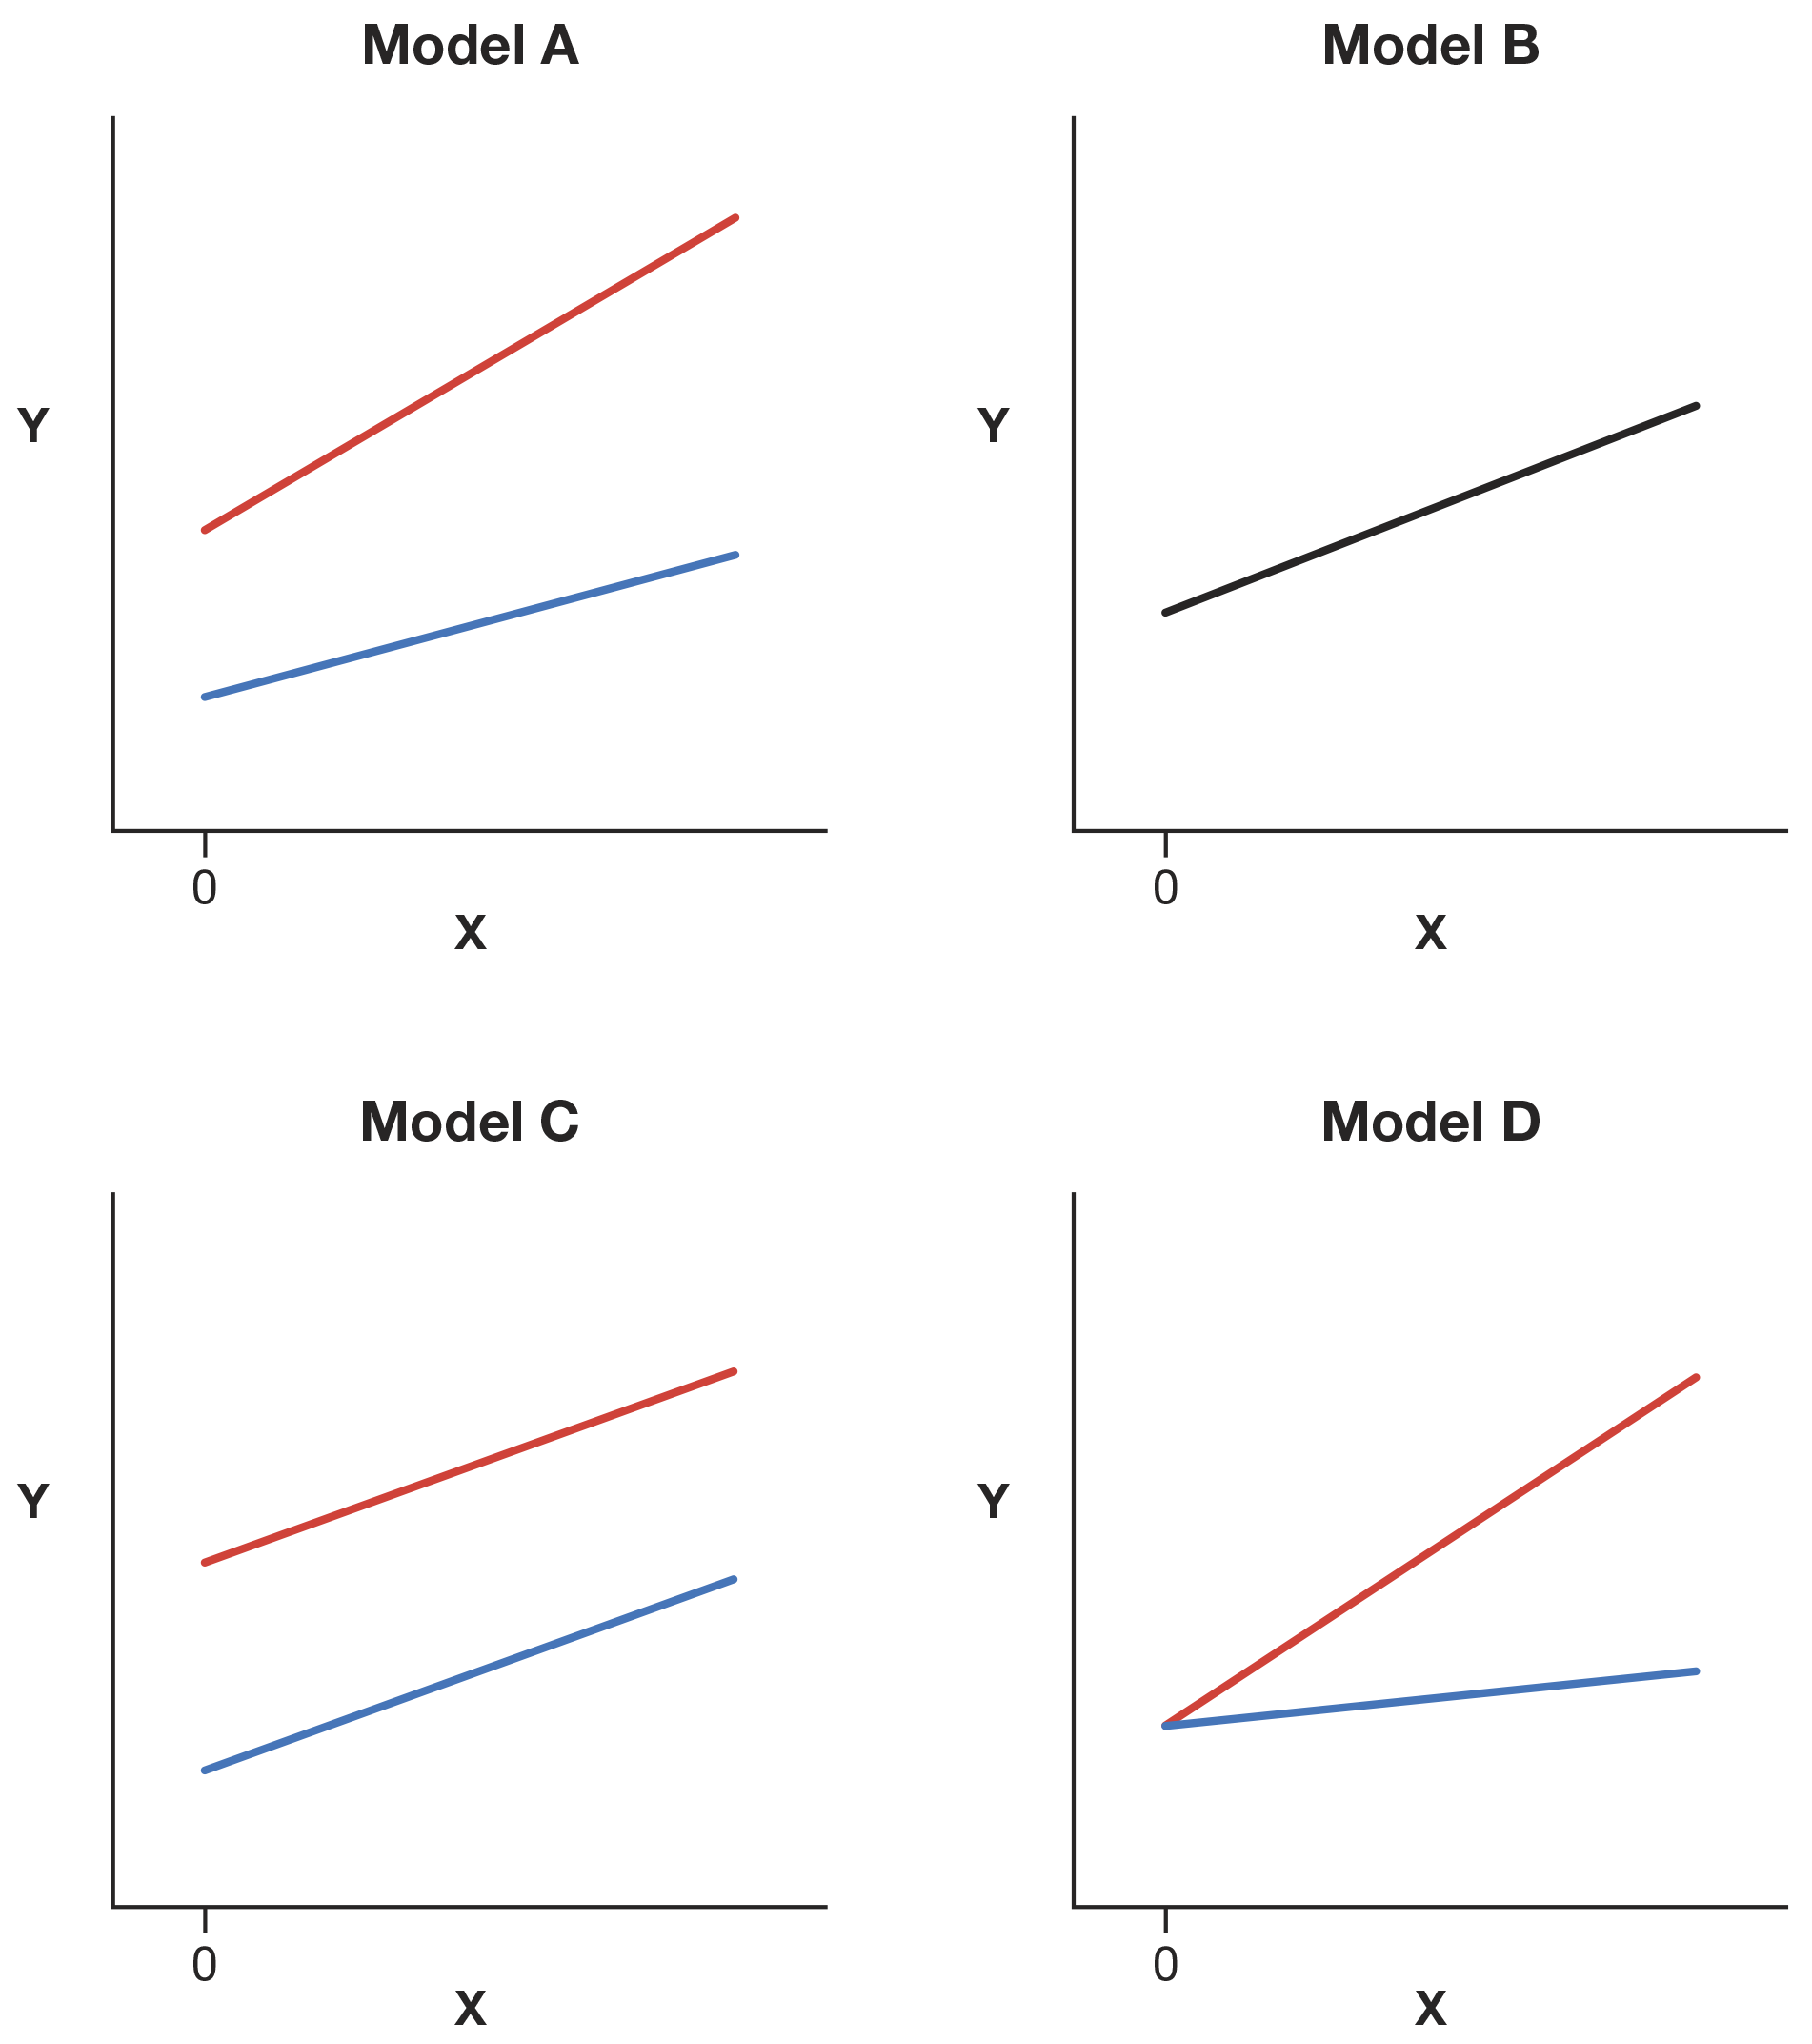
\includegraphics[scale = 0.9]{205940_Slope_Intercept_Graphs_Labels.png} 
\label{Fig. 1}
\caption{Four Models of Interest: (A) Individual intercepts and individual slopes, (B) Single intercept and single slope, (C) Individual intercepts and single slope, (D) Single intercept and individual slopes.}
\end{figure}
\end{center}

\section{Derivation of Sums of Squares for ANOVA Table}
% \bigskip
Following Searle (1971, Chapter 3) let $\mathbf{X}$ be the design matrix for a model of full rank.  The coefficient vector $\mathbf{b}$ has length equal to the column rank of $\mathbf{X}$.  The response vector $\mathbf{y}$ has elements $y_{ij}$, $i = 1, ..., N$. The error vector  $\mathbf{e}$ has elements $e_{ij}$, $i = 1, ..., N $.  Then, in matrix notation,  

\begin{equation}
\mathbf{y} = \mathbf{X}\mathbf{b} + \mathbf{e} , 
\mbox{    with       }
E(\mathbf{y}) =  \mathbf{X}\mathbf{b}. 
\end{equation} 
The solution for the estimation of parameters $\mathbf{b}$ is 
\begin{equation}
\mathbf{\hat{b}} = (\mathbf{X}'\mathbf{X})^{-1}\mathbf{X}\mathbf{y}.
\end{equation}
In this paper, all design matrices are of full column rank.  Therefore, $\mathbf{X}'\mathbf{X} $ is of full rank and $(\mathbf{X}'\mathbf{X})^{-1} $ exists.  

\bigskip

The total sum of squares, SST, uncorrected for the mean, is the sum of: (1) the sum of squares due to regression, SSR, and (2) the sum of squares due to error (to the residuals), SSE (Searle, 1971, pp 93-4).  That is, 

\begin{equation} 
\mbox{SST = SSR + SSE}
\end{equation} 
In matrix notation, this identity is written
\begin{equation}
\mathbf{y}'\mathbf{y} = \mathbf{\hat{b}}'\mathbf{X}'\mathbf{y} + \mathbf{e}'\mathbf{e} = \mathbf{\hat{b}}'\mathbf{X}'\mathbf{X}\mathbf{\hat{b}} + \mathbf{y} ' [\mathbf{I} - \mathbf{X}(\mathbf{X} ' \mathbf{X})^{-1} \mathbf{X} \mathbf{X} '] \mathbf{y}   
\end{equation} 
where $ \mathbf{I} $ is the identity matrix with rank $ N $.  This, in turn, yields
\begin{equation}
\mbox{SSE = SST - SSR} = \mathbf{e} ' \mathbf{e} = \mathbf{y} ' \mathbf{y}  - \mathbf{\hat{b}} ' \mathbf{X} ' \mathbf{y}. 
\end{equation} 

\bigskip
For any given set of observed data, $\mathbf{y}$, for which we want to fit models A, B, C and D, the total (uncorrected) sum of squares $ \mbox{SST}$, or $  \mathbf{y} ' \mathbf{y} $, will be the same.  However, the design matrices, $\mathbf{X} $, the coefficient vectors, $\mathbf{b} $, and the residuals $\mathbf{e} $ will, in general, differ for models A, B, C and D.  

\bigskip

Let $ \mathbf{X_{A}} $,  $  \mathbf{X_{B}}  $, $ \mathbf{X_{C}} $ and $ \mathbf{X_{D}} $ be the design matrices for models A, B, C and D, respectively.  Then, for  model A with design matrix $ \mathbf{X_{A}} $, error vector $ \mathbf{e_{A}} $, and coefficient vector $ \mathbf{b_{A}} $, we have 

\bigskip

\( \mathbf{X_A} =  \left[ \begin{array}{cccc}
1   &  x_{11}   & 0   & 0  \\
1   &  x_{21}   & 0  &  0  \\
\vdots &  \vdots  & \vdots  &  \vdots  \\
1   &  x_{n_{1}1} &  0  & 0  \\
\ldots  & \ldots  & \ldots  & \ldots  \\
0   &   0   &  1   & x_{12}  \\
0   &   0   &  1  & x_{22}   \\
\vdots &  \vdots  & \vdots  &  \vdots  \\
0   &   0   &  1   & x_{n_{2}2}
\end{array} \right] \) ,
\( \mathbf{y} = \left[ \begin{array}{c}
y_{11} \\
y_{21} \\
\vdots  \\
y_{n_{1}1}  \\
\ldots \\
y_{12} \\
y_{22}  \\
\vdots  \\
y_{n_{2}2}
\end{array} \right] \) ,
\( \mathbf{e_{A}} = \left[ \begin{array}{c}
e_{11} \\
e_{21} \\
\vdots  \\
e_{n_{1}1}  \\
\ldots \\
e_{12} \\
e_{22}  \\
\vdots  \\
e_{n_{2}2}
\end{array} \right] \),
\mbox{and}
\( \mathbf{b_{A}} = \left[ \begin{array}{c}
\alpha_{1} \\
\beta_{1}  \\
\alpha_{2}  \\
\beta_{2}
\end{array} \right] \).

\bigskip
\noindent where $ n_{1} + n_{2} = N $. 


\bigskip

\noindent Similarly, for model B, with design matrix $ \mathbf{X_{B}} $, we have
\bigskip

\( \mathbf{X_B} =  \left[ \begin{array}{cccc}
1   &  x_{11}     \\
1   &  x_{21}    \\
\vdots &  \vdots   \\
1   &  x_{n_{1}1}  \\
\ldots  & \ldots    \\
1   & x_{12}  \\
1  & x_{22}   \\
\vdots  &  \vdots  \\
1   & x_{n_{2}2}
\end{array} \right] \) ,
\( \mathbf{y} = \left[ \begin{array}{c}
y_{11} \\
y_{21} \\
\vdots  \\
y_{n_{1}1}  \\
\ldots \\
y_{12} \\
y_{22}  \\
\vdots  \\
y_{n_{2}2}
\end{array} \right] \),
\( \mathbf{e_{B}} = \left[ \begin{array}{c}
e_{11} \\
e_{21} \\
\vdots  \\
e_{n_{1}1}  \\
\ldots \\
e_{12} \\
e_{22}  \\
\vdots  \\
e_{n_{2}2}
\end{array} \right] \) ,
\mbox{and}
\( \mathbf{b_{B}} = \left[ \begin{array}{c}
\alpha \\
\beta 
\end{array} \right] \)

\bigskip
\noindent where, again,  $ n_{1} + n_{2} = N $. 
 
 \bigskip

\noindent For model C, with design matrix $ \mathbf{X_{C}} $, we have
\bigskip

\( \mathbf{X_C} =  \left[ \begin{array}{ccc}
1   &  0  &    x_{11}    \\
1   &  0   &   x_{21}    \\
\vdots &  \vdots  & \vdots   \\
1   &  0  &     x_{n_{1}1}   \\
\ldots  & \ldots  & \ldots    \\
0   &     1   & x_{12}  \\
0   &     1  & x_{22}   \\
\vdots   & \vdots  &  \vdots  \\
0   &     1   &    x_{n_{2}2}
\end{array} \right] \),
\( \mathbf{y} = \left[ \begin{array}{c}
y_{11} \\
y_{21} \\
\vdots  \\
y_{n_{1}1}  \\
\ldots \\
y_{12} \\
y_{22}  \\
\vdots  \\
y_{n_{2}2}
\end{array} \right] \) ,
\( \mathbf{e_{C}} = \left[ \begin{array}{c}
e_{11} \\
e_{21} \\
\vdots  \\
e_{n_{1}1}  \\
\ldots \\
e_{12} \\
e_{22}  \\
\vdots  \\
e_{n_{2}2}
\end{array} \right] \) ,
\mbox{and}
\( \mathbf{b_{C}} = \left[ \begin{array}{c}
\alpha_{1} \\
\alpha_{2}  \\
\beta
\end{array} \right] \).


 \bigskip

\noindent And for model D, with design matrix $ \mathbf{X_{D}} $, we have
\bigskip

\( \mathbf{X_D} =  \left[ \begin{array}{ccc}
1   &  x_{11}    & 0  \\
1   &  x_{21}    &  0  \\
\vdots &  \vdots    &  \vdots  \\
1   &  x_{n_{1}1}   & 0  \\
\ldots  & \ldots  & \ldots   \\
1    &    0    & x_{12}  \\
1    &    0    & x_{22}   \\
\vdots &  \vdots & \vdots  \\
1  &   0     & x_{n_{2}2}
\end{array} \right] \),
\( \mathbf{y} = \left[ \begin{array}{c}
y_{11} \\
y_{21} \\
\vdots  \\
y_{n_{1}1}  \\
\ldots \\
y_{12} \\
y_{22}  \\
\vdots  \\
y_{n_{2}2}
\end{array} \right] \) ,
\( \mathbf{e_{D}} = \left[ \begin{array}{c}
e_{11} \\
e_{21} \\
\vdots  \\
e_{n_{1}1}  \\
\ldots \\
e_{12} \\
e_{22}  \\
\vdots  \\
e_{n_{2}2}
\end{array} \right] \) ,
\mbox{and}
\( \mathbf{b_{D}} = \left[ \begin{array}{c}
\alpha   \\
\beta_{1}  \\
\beta_{2}
\end{array} \right] \).
\bigskip

We have explicitly displayed the design matrices, error (residual) vectors, and coefficient vectors, separately, for models A, B, C and D to drive home the fact that they will differ under each model.  Model A, which fits four parameters, is the full model.  Models B, C, and D are reduced models, which are nested within model A.  Taking $  a_{1}  $, $  b_{1} $, $ a_{2}  $ and $ b_{2}  $  as the least squares estimates of $ \alpha_{1} $, $ \beta_{1} $, $ \alpha_{2}  $ and $ \beta_{2}  $, respectively,  the sum of squares due to regression for model A is 


\begin{equation}
\mathbf{SSR_{A}} = \mbox{SS} (a_{1}, b_{1},  a_{2}, b_{2}) =  \mathbf{\hat{b_{A}}} ' 
\mathbf{X_{A}} ' \mathbf{X_{A}} \mathbf{\hat{b_{A}}} = \mathbf{\hat{b_{A}}} '  \mathbf{X_{A}} ' \mathbf{y} . 
\end{equation} 
% \bigskip
Letting $  a $ and $  b $ represent the estimates for $ \alpha  $ and $ \beta  $,  the sum of squares due to regression for model B is 

\begin{equation}
\mathbf{SSR_{B}} = \mbox{SS} (a, b) =  \mathbf{\hat{b_{B}}} ' 
\mathbf{X_{B}} ' \mathbf{X_{B}} \mathbf{\hat{b_{B}}} = \mathbf{\hat{b_{B}}} '  \mathbf{X_{B}} ' \mathbf{y} . 
\end{equation}
Taking $ a_{1}  $, $ a_{2}  $ and $ b  $ as the least squares estimates for $ \alpha_{1}  $,  $  \alpha_{2} $ and $  \beta $, the sum of squares due to regression for model C is 

\begin{equation}
\mathbf{SSR_{C}} = \mbox{SS} ( a_{1},  a_{2}, b) =  \mathbf{\hat{b_{C}}} ' 
\mathbf{X_{C}} ' \mathbf{X_{C}} \mathbf{\hat{b_{C}}} = \mathbf{\hat{b_{C}}} '  \mathbf{X_{C}} ' \mathbf{y} . 
\end{equation} 
Finally, letting $ a  $,  $  b_{1}  $ and  $  b_{2}  $ be the least squares estimates of $  \alpha  $, $  \beta_{1} $ and $  \beta_{2}  $, the sum of squares due to regression for model D is 

\begin{equation}
\mathbf{SSR_{D}} = \mbox{SS} (a, b_{1}, b_{2}) =  \mathbf{\hat{b_{D}}} ' 
\mathbf{X_{D}} ' \mathbf{X_{D}} \mathbf{\hat{b_{D}}} = \mathbf{\hat{b_{D}}} '  \mathbf{X_{D}} ' \mathbf{y} . 
\end{equation} 

\bigskip
As stated above, for any given set of criterion data, $\mathbf{y}$, for which we want to fit models A, B, C and D, the total (uncorrected) sum of squares $ \mbox{SST}$, or $  \mathbf{y} ' \mathbf{y} $, will remain the same.  It is also true that the predictor (regressor) variables, $ x_{ij} $'s, will remain the same, though they are grouped differently in the design matrices for each model.   The design matrices, $\mathbf{X} $, the estimated coefficient vectors, $\mathbf{\hat{b}} $, and the residuals $\mathbf{e} $ will, in general, differ among models A, B, C and D.  For example, the values of $ a_{1}  $ and $ a_{2}  $ in (12) will \emph{not}, in general, be equal to the values of $ a_{1}  $ and $ a_{2}  $ in (14).  The value of $ a $ in (13) will not be equal (in general) to $ a $ in (15), nor will the value of $ b  $ in (13) be equal to $ b $ in (14).  

\bigskip

From equation (9), we have $ \mbox{SST} = \mbox{SSR} + \mbox{SSE}  $.  Table 1 shows the ANOVA source table for models A, B, C and D.  The number of parameters estimated in model A is 4. The numbers of parameters estimated in models B, C and D, respectively, are 2, 3, and 3.   The $ \mbox{SST} = \mathbf{y}'\mathbf{y} $ does not change for a particular data set.  Since 4 parameters are estimated in model A, the sum of squares for regression for model A, $ \mathbf{SSR_{A}} $, necessarily (of necessity) must be greater than or equal to the sum of squares due to regression for models B, C, and/or D.  That is $ \mathbf{SSR_{A}} \geq \mathbf{SSR_{B}} $, $ \mathbf{SSR_{A}} \geq \mathbf{SSR_{C}} $, and $ \mathbf{SSR_{A}} \geq \mathbf{SSR_{D}} $.  At the same time, it must be true that the residual sum of squares for model A, $ \mathbf{SSE_{A}} $, must be less than or equal to the residuals sums of squares for models B, C, or D.  That is $ \mathbf{SSE_{A}} \leq \mathbf{SSE_{B}} $, $ \mathbf{SSE_{A}} \leq \mathbf{SSE_{C}} $, and $ \mathbf{SSE_{A}} \leq \mathbf{SSE_{D}} $.       

\bigskip
       

\bigskip

\begin{table} [h]
\centerline{Table 1: ANOVA Source Table for Models A, B, C and D} 
\centering
\bigskip
\begin{tabular}{cccccc}
Model & No. Parms & Resid & SST & SSR & SSE \\ 
          & Estimated &   df   &   &    & \\
\hline
    &    &     &    &    &  \\
\textbf{A}  &  4  &  $ N - 4 $  &  $  \mathbf{y} ' \mathbf{y} $  & $ \mathbf{SSR_{A}} = \mathbf{b_{A}}'\mathbf{X_{A}}'\mathbf{y} $ &   $ \mathbf{SSE_{A}} =  \mathbf{y} ' \mathbf{y} - \mathbf{b_{A}}'\mathbf{X_{A}}'\mathbf{y}    $        \\
 &  &  &  &  &  \\
\textbf{B}  &  2  &  $ N - 2 $  &  $  \mathbf{y} ' \mathbf{y} $  & $ \mathbf{SSR_{B}} = \mathbf{b_{B}}'\mathbf{X_{B}}'\mathbf{y} $ &   $  \mathbf{SSE_{B}} =  \mathbf{y} ' \mathbf{y} - \mathbf{b_{B}}'\mathbf{X_{B}}'\mathbf{y}    $        \\
&  &  &  &  &  \\
\textbf{C}  &  3  &  $ N - 3 $  &  $  \mathbf{y} ' \mathbf{y} $  & $ \mathbf{SSR_{C}} = \mathbf{b_{C}}'\mathbf{X_{C}}'\mathbf{y} $ &   $  \mathbf{SSE_{C}} = \mathbf{y} ' \mathbf{y} - \mathbf{b_{C}}'\mathbf{X_{C}}'\mathbf{y}    $        \\
&  &  &  &  &  \\
\textbf{D}  &  3  &  $ N - 3 $  &  $  \mathbf{y} ' \mathbf{y} $  & $ \mathbf{SSR_{D}} = \mathbf{b_{D}}'\mathbf{X_{D}}'\mathbf{y} $ &   $  \mathbf{SSE_{D}} = \mathbf{y} ' \mathbf{y} - \mathbf{b_{D}}'\mathbf{X_{D}}'\mathbf{y}    $        \\
\end{tabular} 
\end{table}

\bigskip


\section{The Extra Sum of Squares Principle and Tests for Parameters Being Zero}

Recall that $ \mathbf{SSR_{A}} = \mbox{SS} (a_{1}, b_{1}, a_{2}, b_{2})  $ to denote the regression sum of squares for the full model, model A.  Similarly, for the completely reduced model B, we write $ \mathbf{SSR_{B}} = \mbox{SS} (a, b) $.  The regression sum of squares for the reduced model C is written $ \mathbf{SSR_{C}} = \mbox{SS} (a_{1}, a_{2}, b) $ and the regression sum of squares for the reduced model D is written $ \mathbf{SSR_{D}} = \mbox{SS} (a, b_{1}, b_{2})  $. As stated previously, none of the estimated values in model A, $  (a_{1}, b_{1}, ...)   $, etc., will, in general, be equal to any of the estimates of $ a_{1}, b_{1}  $, etc., in models B, C or D.  

\vspace{2 mm}

In the regression analysis of the two-group, straight-line ANCOVA setup, there are typically three null hypotheses of interest that arise in connection with comparisons among these four models.  These are referred to as the null hypotheses for: (1) \emph{equivalent data sets}, (2) \emph{equivalent slopes}, and (3) \emph{equivalent intercepts}.  Under standard assumptions, tests for acceptance or rejection of these null hypotheses can be accomplished using the \emph{reduction in sums of squares} principle (Searle, 1971, pp 116-20, pp 246-9), the \emph{extra sum of squares} principle (Draper and Smith, 1998, pp 149-51), or the \emph{incremental sum of squares} principle (Fox, 2008, pp 158-9).  It can be shown (e.g., Searle, 1971, pp 99-102, pp 246-9) that under assumptions of the equivalence of specific parameters in the models being compared, the expected value of the difference in the regression sums of squares between the full model (estimating $ p $ parameters) and a reduced model (estimating $ q $ parameters), appropriately modified by their degrees of freedom ($ p - q $) to yield mean squares, are equal to $ \sigma^{2} $.  In addition, if the errors are normally distributed, then their difference is distributed as  $ \sigma^{2} \chi^{2}_{(p-q)}  $ independently of $ s^{2}  $.  This means that the mean squares can be compared to $ \sigma^{2} $ with an $ F (p-q, \nu) $ test, where $ \nu $ is the number of degrees of freedom on which $ \sigma^{2} $ is based, i.e., on the Mean Square Error (MSE), or $ s^{2} $, for model A.    

\vspace{2 mm}

We discuss the tests for each of these null hypotheses in turn.     

% (Searle, 1971, p. 32, p. 48, pp 99-102, pp 246-9; Draper and Smith, 1998, pp 149-51; Fox, 2008, pp 158-9)

\subsection{Test for Equivalence of Data Sets} 
Model A represents the full model. It fits four parameters $  (\alpha_{1}, \beta_{1}, \alpha_{2}, \beta_{2}) $. Model B is a reduced model; it fits only two parameters $  (\alpha,  \beta) $. The null hypothesis  of \emph{equivalent data sets}, is (states) that the data under consideration, which are designated by two nominally distinct groups and which require two intercepts and two slopes in model A, can be more parsimoniously explained by being fit with a single intercept and slope in model B. A test for acceptance or rejection of the null hypothesis of equivalent data sets can be accomplished using the \emph{extra sum of squares} principle. Let the regression sum of squares for model A be denoted as $ \mathbf{SSR_{A}} $ and regression sum of squares for model B be denoted as $ \mathbf{SSR_{B}} $.  Then $ \mathbf{SSR_{A}} -  \mathbf{SSR_{B}} $ is the extra sum of squares due to the inclusion of two intercepts and slopes in model A over the inclusion of a single intercept and slope in model B. $ \mathbf{SSR_{A}} $ is obtained by estimating $ p = 4 $ parameters, yielding $ (N - p)  = (N - 4) $ residual degrees of freedom.  $  \mathbf{SSR_{B}} $ is obtained by estimating $ q = 2 $ parameters, thus yielding $  (N - q) = (N - 2)  $ residual degrees of freedom.  The test for $ \mathbf{SSR_{A}} -  \mathbf{SSR_{B}} $, therefore,  has $  p - q = 4 - 2 = 2  $ degrees of freedom.  It can be shown (Searle, pp 99-102; Draper and Smith, pp 149-51) that if $ \alpha_{1} = \alpha_{2} $    and  $  \beta_{1} = \beta_{2}   $ then $ E\{  \mathbf{SSR_{A}} -  \mathbf{SSR_{B}}   / (p - q = 2) \} = \sigma^{2} $.  In addition, if the errors are normally distributed, then $ \mathbf{SSR_{A}} -  \mathbf{SSR_{B}} $ is distributed as  $ \sigma^{2} \chi^{2}_{(p-q=2)}  $ independently of $ s^{2}  $.  Hence, the mean square $ \mathbf{MSR_{(A-B)}}  =  \{  \mathbf{SSR_{A}} -  \mathbf{SSR_{B}}   / (p - q = 2) \} $, can be compared to $ \sigma^{2} $ with an $ F (p-q =2, \nu) $ test, where $ \nu $ is the number of degrees of freedom on which $ \sigma^{2} $ is based, i.e., on the Mean Square Error (MSE), for model A, designated as $ \mathbf{MSE_{A}} $, or $  s^2 $.  

\vspace{2 mm}

In an alternative formulation (Draper and Smith, p. 151), we arrive at the same conclusion by considering the residual sums of squares for each model instead of the regression sums of squares.  The quantity $ \mathbf{ SSE_{B}} - \mathbf{SSE_{A} }  =   \mathbf{SSR_{A}} -  \mathbf{SSR_{B}}  $, and thus, in an obvious notation, $ \mathbf{ MSE_{(B-A)}}   =  \mathbf{MSR_{(A-B)}} $, and the $  F  $ statistic is computed exactly as described above.
\bigskip

\subsection{Test for Equivalence of Slopes}
Again, model A represents the full model; it fits four parameters $  (\alpha_{1}, \beta_{1}, \alpha_{2}, \beta_{2}) $. Model C is a reduced model that fits the data with two intercepts and a single slope common to both groups.  Therefore, it fits only three parameters $  (\alpha_{1},  \alpha_{2}, \beta)  $.  The null hypothesis of interest here, the hypothesis of \emph{equivalent slopes}, is that the data under consideration, which are designated by two nominally distinct groups, and which require two intercepts and two slopes in model A, can be more parsimoniously explained by a model that requires two distinct intercepts, but only a single slope common to both groups, i.e., model C.  A test for acceptance or rejection of the null hypothesis of equivalent slopes can be accomplished using the \emph{extra sum of squares} principle. As before, let the regression sum of squares for model A be denoted as $ \mathbf{SSR_{A}} $ and regression sum of squares for model C be denoted as $ \mathbf{SSR_{C}} $. Then $ \mathbf{SSR_{A}} -  \mathbf{SSR_{C}} $ is the extra sum of squares due to the inclusion of two separate intercepts and slopes in model A over the inclusion of two intercepts and a single slope in model C. Since  $ \mathbf{SSR_{A}} $ is fit with $ p = 4 $ parameters (yielding $ (N - p) = (N - 4) $ residual degrees of freedom) and  $  \mathbf{SSR_{C}} $ is fit with $ q = 3 $ parameters (yielding $  (N - q) = (N - 3) $ residual degrees of freedom), then the test for $ \mathbf{SSR_{A}} -  \mathbf{SSR_{C}} $ has $  p - q = 4 - 3 = 1  $ degree of freedom.  If $ \beta_{1} = \beta_ {2} $ then $ E\{  \mathbf{SSR_{A}} -  \mathbf{SSR_{C}}   / (p - q = 1) \} = \sigma^{2} $ (Searle, 1971).  If the errors are normally distributed, then $ \mathbf{SSR_{A}} -  \mathbf{SSR_{C}} $ is distributed as  $ \sigma^{2} \chi^{2}_{(p-q=1)}  $ independently of $ s^{2}  $.  Thus, $ \{  \mathbf{SSR_{A}} -  \mathbf{SSR_{C}}   / (p - q = 1) \} $ can be compared to $ \sigma^{2} $ with an $ F_(p-q =1, \nu) $ test, where $ \nu $ is the number of degrees of freedom on which $ \sigma^{2} $ is based, i.e., the Mean Square Error (MSE) for model A, or $  s^2 $.  
\vspace{2 mm}
 
With an alternative formulation (Draper and Smith, p. 151), we arrive at the same conclusion by considering the residual sums of squares for each model instead of the regression sums of squares.  The quantity $ \mathbf{ SSE_{C}} - \mathbf{SSE_{A} }  =   \mathbf{SSR_{A}} -  \mathbf{SSR_{C}}  $, and thus, in an obvious notation, $ \mathbf{ MSE_{(C-A)}}   =  \mathbf{MSR_{(A-C)}} $, and the $  F  $ statistic is computed exactly as described above.
\bigskip
   
\subsection{Test for Equivalence of Intercepts}
Again, model A represents the full model; it fits four parameters $  (\alpha_{1}, \beta_{1}, \alpha_{2}, \beta_{2}) $.  Model D is a reduced model that fits the data with a single, common intercept and two distinct slopes.  It fits only three parameters $  (\alpha, \beta_{1}, \beta_{2}) $. The null hypothesis of interest here, the hypothesis of \emph{equivalent intercepts}, is that the data which are designated by two nominally distinct groups, and which require two distinct intercepts and two distinct slopes, can be more parsimoniously explained by a model that requires only a single intercept, but with two distinct slopes.  A test for acceptance or rejection of the null hypothesis of equivalent intercepts can again be accomplished using the \emph{extra sum of squares} principle. Let the regression sum of squares for model A be denoted as $ \mathbf{SSR_{A}} $ and the regression sum of squares for model D be denoted as $ \mathbf{SSR_{D}} $. Then $ \mathbf{SSR_{A}} -  \mathbf{SSR_{D}} $ is the extra sum of squares due to the inclusion of two separate intercepts and slopes in model A over the inclusion of a single intercept and two distinct slopes in model D. Since  $ \mathbf{SSR_{A}} $  is fit with $ p = 4 $ parameters (and yields $ (N - P) = (N - 4) $ residual degrees of freedom) and $  \mathbf{SSR_{D}} $ is fit with $ q = 3 $ parameters (and yields $ (N - p) = (N - 3) $ residual degrees of freedom), then the test for $ \mathbf{SSR_{A}} -  \mathbf{SSR_{D}} $ has $  p - q = 4 - 3 = 1  $ degree of freedom.  If $ \alpha_{1} = \alpha_ {2} $ then $ E\{  \mathbf{SSR_{A}} -  \mathbf{SSR_{D}}   / (p - q = 1) \} = \sigma^{2} $, and if the errors are normally distributed, then $ \mathbf{SSR_{A}} -  \mathbf{SSR_{C}} $ is distributed as  $ \sigma^{2} \chi^{2}_{(p-q=1)}  $ independently of $ s^{2}  $.  Hence, $ \{  \mathbf{SSR_{A}} -  \mathbf{SSR_{D}}   / (p - q = 1) \} $ can be compared to $ \sigma^{2} $ with an $ F_(p-q =1, \nu) $ test, where $ \nu $ is the number of degrees of freedom on which $ \sigma^{2} $ is based, i.e., the Mean Square Error (MSE) for Model A, or $  s^2 $.   

\vspace{2 mm}

In an alternative formulation (Draper and Smith, p. 151), we arrive at the same conclusion by considering the residual sums of squares for each model instead of the regression sums of squares.  The quantity $ \mathbf{ SSE_{D}} - \mathbf{SSE_{A} }  =   \mathbf{SSR_{A}} -  \mathbf{SSR_{D}}  $, and thus, in an obvious notation, $ \mathbf{ MSE_{(D-A)}}   =  \mathbf{MSR_{(A-D)}} $, and the $  F  $ statistic is computed exactly as described above.
\bigskip
  

\bigskip 
\bigskip

\subsection{Analyses of Variance}
Table 2 shows (displays) a composite ANOVA source table for the tests of differences between model A and reduced models B, C, and D, respectively.  In the first three major `rows' in the ``Source of Variation'' column (separated by double lines), we list the source of variation as being comprised of two quantities: (1) the variation due to the estimated parameters in the full model, i.e., $ a_{1} $, $ b_{1}  $, $  a_{2} $, and $  b_{2} $, `over' (2) the variation due to the estimated parameters in the corresponding reduced model of interest.  The term `over' in this context means that we determine the variation due to the estimated parameters in the full model A, `over and above' or `after' determining the variation due to the estimated parameters in the corresponding reduced model of interest, B, C or D.   For example, in the second major `row', which deals with the comparison of models A and C, we describe the source of variation as $ (a_{1}, b_{1}, a_{2}, b_{2})  $ over $  (a_{1}, a_{2}, b)  $.  The \emph{difference} in the sums of squares can be formulated in two different, but equivalent, ways: (1) as the difference in the sums of squares due to \emph{regression}, or (2) as the difference in the sums of squares due to \emph{error} (\emph{residual}).  Thus, in the first `sub-row' in the ``Sum of Squares'' column, we have the $ \mathbf{SSR_{A}} - \mathbf{SSR_{B}}  $. In our ANCOVA setup, the $ \mathbf{SSR_{A}}  $ is obtained by fitting four parameters to the data.  The  $ \mathbf{SSR_{B}}  $ is obtained by fitting three parameters to the same data.  Of necessity, the  $ \mathbf{SSR_{A}} \leq \mathbf{SSR_{B}}  $.   In the second `sub-row' of the second major `row', we have in the ``Sum of Squares'' column $ \mathbf{SSE_{B}} - \mathbf{SSE_{A}}  $.  Necessarily, the  $ \mathbf{SSE_{B}} \leq \mathbf{SSE_{A}}  $, and this value is identically equivalent to $ \mathbf{SSR_{A}} - \mathbf{SSR_{B}}  $. That is, $ \mathbf{SSR_{A}} - \mathbf{SSR_{B}}  \equiv  \mathbf{SSE_{B}} - \mathbf{SSE_{A}}  $.  This is due to the fact that both models A and C are of full rank and are being fit to the same data and that SST = SSR + SSE, regardless of the model being fit. 

  

\vspace{2 mm}

The ``Degrees of Freedom'' column displays the degrees of freedom associated with the hypothesis of interest.  This is equal to the number of parameters fit under model A, $  Np(A) $, minus the number of parameters under the reduced model, $  Np(RM) $, where `$RM$' is `$A$', `$B$' or `$C$'.  In our ANCOVA setup, degrees of freedom associated with the difference between model A and model B is $  Np(A) - Np(B) = 2  $.  The degrees of freedom associated with the difference between model A and model C is $  Np(A) - Np(C) = 1  $.  And the degrees of freedom associated with the difference between model A and model D is $  Np(A) - Np(D) = 1  $.  The ``Mean Square'' column displays the sums of squares divided by their respective degrees of freedom.  

\vspace{2 mm}

The ``Mean Square'' column displays the sums of squares divided by their respective degrees of freedom.  

The central chi-square distribution is denote by $ \chi^{2}  $ distribution . . . 

The non-central chi-square distribution is denoted by $ \chi^{2'} $ ... distribution . . . 


The ``$F$ Statistic'' column displays the relevant $F$ statistic for the hypothesis of interest.  It can be shown (Searle, 1971, p. 174) that the mean square for the residual term $ \mathbf{MSE_{A}}  $

 for the three major `rows' of Table 2      

\vspace{2 mm}

The final row under the ``Source of Variation'' column in Table 2 the entry `Residual' represents the error, or residual, variation for the ANCOVA problem.  Its degrees of freedom, $ \nu $, is equal to the number of cases in the data set minus the number of parameters estimated in model A, or $ [N - Np(A)]  $, which is equal to $ N - 4  $.  The sum of squares associated with residual variation is $ \mathbf{SSE_{A}} =  \mathbf{y'y} - \mathbf{SSR_{A}}  $ and the mean square for error, $ \mathbf{MSE_{A}}  $, is the residual sum of squares divided by it degrees of freedom, or $  \mathbf{SSE_{A}} / \nu $.    
                            
\bigskip

\bigskip
 \begin{table} [h]
\centerline{Table 2:  ANOVA Source Table for Tests of Differences Between} 
\centerline{Reduced Models B, C, and D Against the Full Model A } 
\centering
\bigskip
\begin{tabular}{ccccc}
\hline
Source of  &   Degrees of & Sum of     & Mean     & $ F $ \\ 
Variation   &   Freedom    & Squares   & Square  &  Statistic \\
\hline
\hline
\bigskip
$ (a_{1}, b_{1}, a_{2}, b_{2}) $    &    $ Np(A) - Np(B)  $    &    $  \mathbf{SSR_{A}} -  \mathbf{SSR_{B}} $ &  $ (\mathbf{SSR_{A}} -  \mathbf{SSR_{B}})/2 $    &    $ \mathbf{MSR_{(A-B)}} / \mathbf{MSE_A} $   \\
over $  (a, b)  $  &  $ 2 $   &    $ \mathbf{SSE_{B}} -  \mathbf{SSE_{A}} $    &     $ (\mathbf{SSE_{B}} -  \mathbf{SSE_{A}})/2 $   &  $    \mathbf{MSE_{(B-A)}} /           \mathbf{MSE_A} $   \\
\hline
\hline
\bigskip
$ (a_{1}, b_{1}, a_{2}, b_{2}) $    &    $ Np(A) - Np(C)  $    &    $  \mathbf{SSR_{A}} -  \mathbf{SSR_{C}} $ &  $ (\mathbf{SSR_{A}} -  \mathbf{SSR_{C}})/1 $    &    $ \mathbf{MSR_{(A-C)}} / \mathbf{MSE_A} $  \\
over $  (a_{1}, a_{2},  b)  $  &  $ 1 $   &    $ \mathbf{SSE_{C}} -  \mathbf{SSE_{A}} $    &     $ (\mathbf{SSE_{C}} -  \mathbf{SSE_{A}})/1  $   &  $ \mathbf{MSE_{(C-A)}} / \mathbf{MSE_A} $    \\
\hline 
\hline
\bigskip
$ (a_{1}, b_{1}, a_{2}, b_{2}) $    &    $ Np(A) - Np(D)  $    &    $  \mathbf{SSR_{A}} -  \mathbf{SSR_{D}} $ &  $ (\mathbf{SSR_{A}} -  \mathbf{SSR_{D}})/1 $    &    $ \mathbf{MSR_{(A-D)}} / \mathbf{MSE_A} $  \\
% \vspace{2 mm} % this puts the space after 'over (a, b1, b2)
over $  (a, b_{1}, b_{2})  $  &  $ 1 $   &    $ \mathbf{SSE_{D}} -  \mathbf{SSE_{A}} $    &     $ (\mathbf{SSE_{D}} -  \mathbf{SSE_{A}})/1  $   &  $ \mathbf{MSE_{(D-A)}} / \mathbf{MSE_A} $    \\
\hline 
\hline
\bigskip
\vspace{2 mm} % this line puts the space after 'Residual' 
Residual &  $ \nu = [N - Np(A)] $  &  $ \mathbf{SSE_{A}} =   \mathbf{y'y} - \mathbf{SSR_{A}}  $ &  $ \mathbf{MSE_A} =  \mathbf{SSE_{A}} / \nu $ &   ---  \\
\hline
\end{tabular} 
\end{table}
\bigskip

\section{Example}
Suppose have 10 observations, two sets of five observations in two groups. Hence, \(\mathbf{y'} = \left[ \begin{array}{ccccccccccc}4 & 7 & 8 & 11 & 15 & | & 14 & 17 & 18 & 21 & 24  \end{array} \right]\).  The $ | $ symbol represents the distinction between the two groups. Let let the regressors be \(\mathbf{x'} = \left[ \begin{array}{ccccccccccc}1 & 2 & 3 & 4 & 5 & | & 1 & 2 & 3 & 4 & 5  \end{array} \right]\).  When we fit models A, B, C and D to these data, we produce the outcomes reported in Table 3. The total sum of squares, uncorrected for the mean, SST, is $  \mathbf{y} ' \mathbf{y} = 2301  $.  This value does not change for the four models in this example.  However, the sums of squares due to regression, SSR, and the sums of squares to error (residual), SSE, \emph{do} change in each of the models.       
\bigskip
\vspace{2 mm}

In model A, the sum of squares due to regression (SSR) is $ \mathbf{SSR_{A}} = 2297.40 $, while the sum of squares due to error (SSE) is $ \mathbf{SSE_{A}} = 3.60 $. These two sums of squares add up to the total sum of squares (SST), which is  $ \mathbf{y'y} = 2301.  $  In model C, for example, the sum of squares due to regression (SSR) is $ \mathbf{SSR_{C}} = 2297.20 $, while the sum of squares due to error (SSE) is $ \mathbf{SSE_{C}} = 3.80 $. These two sums of squares again add up to the total sum of squares (SST), which is  $ \mathbf{y'y} = 2301.  $  

\bigskip

\begin{table} [h]
\centerline{Table 3: ANOVA Source Table for Example Data} 
\centering
\bigskip
\begin{tabular}{cccccr}
Model & No. Parms & Resid & SST & SSR & SSE \\ 
          & Estimated &   df   &   &    & \\
\hline
    &    &     &    &    &  \\
\textbf{A}  &  4  &  $ 6 $  &  $  \mathbf{y} ' \mathbf{y} = 2301 $  & $ \mathbf{SSR_{A}} = 2297.40 $ &   $ \mathbf{SSE_{A}} =  3.60    $        \\
 &  &  &  &  &  \\
\textbf{B}  &  2  &  $ 8 $  &  $  \mathbf{y} ' \mathbf{y} = 2301 $  & $ \mathbf{SSR_{B}} = 2751.10 $ &   $  \mathbf{SSE_{B}} =  243.90   $        \\
&  &  &  &  &  \\
\textbf{C}  &  3  &  $ 7 $  &  $  \mathbf{y} ' \mathbf{y} = 2301 $  & $ \mathbf{SSR_{C}} = 2297.20 $ &   $  \mathbf{SSE_{C}} = 3.80    $        \\
&  &  &  &  &  \\
\textbf{D}  &  3  &  $ 7 $  &  $  \mathbf{y} ' \mathbf{y} = 2301 $  & $ \mathbf{SSR_{D}} = 2248.24 $ &   $  \mathbf{SSE_{D}} = 52.76    $        \\
\end{tabular} 
\end{table}

Next, we perform the tests for the three hypotheses of interest.  In Table 4, the difference in the sum of squares due to regression for model A and the sum of squares due to regression for model B, $  \mathbf{SSR_{A}} -  \mathbf{SSR_{B}} $, is denoted as $  \mathbf{SSR_{(A-B)}}  $.  Similarly, the difference in the sum of squares due to error for model B and the sum of squares due to error for model A, $  \mathbf{SSE_{B}} -  \mathbf{SSE_{A}}   $, and is denoted as $ \mathbf{ SSE_{(B-A)}}   $. These quantities are equal.  That is $   \mathbf{SSR_{(A-B)}}  =  \mathbf{ SSE_{(B-A)}}   $.  The degrees of freedom associated with the difference between model A and model B is $  Np(A) - Np(B)  $.  In this paper it is always true that $  Np(A) = 4 $ and $  Np(B) = 2  $.  Hence, for the problem considered here,  $  Np(A) - Np(B)   =  (4 - 2) =  2$.  The difference in the sums of squares for models A and B due to, say, regression is $ \mathbf{SSR_{(A-B)}}  = 240.30 $.  This is identical to the the difference in the sums of squares due to error for models A and B, $  \mathbf{SSE_{(B-A)}} $. The mean square for the difference between models A and B, $ \mathbf{MSR_{(A-B)}}  $ is $ \mathbf{SSR_{(A-B)}} / 2 = 240.30/2 = 120.15 $.  The $ F  $ statistic is obtained by taking dividing the mean square due to regression by the mean square for error for model A, $ \mathbf{MSR_{(A-B)}} / \mathbf{MSE_{A}} = 120.15/ 0.6 = 200.25 $.  



\vspace{2 mm}

Taking another example, the difference in the sum of squares due to regression for model A and the sum of squares due to regression for model C, $  \mathbf{SSR_{A}} -  \mathbf{SSR_{C}} $, is denoted as $  \mathbf{SSR_{(A-C)}}  $.  Similarly, the difference in the sum of squares due to error for model C and the sum of squares due to error for model A, $  \mathbf{SSE_{C}} -  \mathbf{SSE_{A}}   $, and is denoted as $ \mathbf{ SSE_{(C-A)}}   $. These are equivalent; hence $   \mathbf{SSR_{(A-C)}}  =  \mathbf{ SSE_{(C-A)}}   $.  The degrees of freedom associated with the difference between model A and model C is $  Np(A) - Np(C)  $.  In this paper it is always true that $  Np(A) = 4 $ and $  Np(C) = 3  $.  Hence,  $  Np(A) - Np(C)   =  (4 - 3) =  1$.  The difference in the sums of squares for models A and C due to regression is $ \mathbf{SSR_{(A-C)}}  = 0.20 $, which is identical to the the difference in the sums of squares due to error for models A and C, $  \mathbf{SSE_{(C-A)}} $. The mean square for the difference between models A and C, $ \mathbf{MSR_{(A-C)}}  $ is $ \mathbf{SSR_{(A-C)}} / 1 = 0.20/1 = 0.20 $.  The $ F  $ statistic is obtained by taking dividing the mean square due to regression by the mean square for error for model A, $ \mathbf{MSR_{(A-C)}} / \mathbf{MSE_{A}} = 0.20 / 0.6 = 0.33 $.     

 \begin{table} [h]
\centerline{Table 4:  ANOVA Source Table for Tests of Differences Between} 
\centerline{Reduced Models B, C, and D Against the Full Model A  with Example Data} 
\centering
\bigskip
\begin{tabular}{ccccc}
\hline
Source of  &   Degrees of & Sum of     & Mean     & $ F $\\ 
Variation   &   Freedom    & Squares   & Square  &  Statistic \\
\hline
\hline
\bigskip
$ (a_{1}, b_{1}, a_{2}, b_{2}) $    &    $ Np(A) - Np(B)  $    &    $  \mathbf{SSR_{(A-B)}} = 240.30 $ &  $ \mathbf{MSR_{(A-B)}} =  120.15 $    &    $ \mathbf{F_{reg_{(A-B)}}} = 200.25 $   \\
over $  (a, b)  $  &  $ 2 $   &    $ \mathbf{ SSE_{(B-A)}} = 240.30 $    &     $ \mathbf{MSE_{(B-A)}} = 120.15  $   &  $    \mathbf{F_{err_{(B-A)}}} = 200.25 $   \\
\hline
\hline
\bigskip
$ (a_{1}, b_{1}, a_{2}, b_{2}) $    &    $ Np(A) - Np(C)  $    &    $   \mathbf{SSR_{(A-C)}} = 0.20 $ &  $ \mathbf{MSR_{(A-C)}} =  0.20  $    &    $ \mathbf{F_{reg_{(A-C)}}} = 0.33  $  \\
over $  (a_{1}, a_{2},  b)  $  &  $ 1 $   &    $ \mathbf{SSE_{(C-A)}} = 0.20 $ &  $ \mathbf{MSE_{(C-A)}} =  0.20  $   &  $  \mathbf{F_{err_{(C-A)}}} = 0.33 $    \\
\hline 
\hline
\bigskip
$ (a_{1}, b_{1}, a_{2}, b_{2}) $    &    $ Np(A) - Np(D)  $    &    $  \mathbf{SSR_{(A-D)}} = 49.16 $ &  $ \mathbf{MSR_{(A-D)}} =  49.16 $    &    $ \mathbf{F_{reg_{(A-D)}}} = 81.94 $  \\
over $  (a, b_{1}, b_{2})  $  &  $ 1 $   &    $ \mathbf{SSE_{(D-A)}} = 49.16 $ &  $ \mathbf{MSE_{(D-A)}} =  49.16  $   &  $  \mathbf{F_{err_{(D-A)}}} = 81.94  $    \\
\hline 
\hline
\bigskip
Residual &  $ \nu = [N - Np(A)] $  &  $  \mathbf{y} ' \mathbf{y} - \mathbf{SSR_{A}}  $ &  $ \mathbf{MSE_A} $ &   ---  \\
        &  (10 - 4)  = 6   & (2301 -  2297.4) = 3.6 &  = 0.6   & --- \\  
\hline
\end{tabular} 
\end{table}
\bigskip

Table 5 simplifies Table 4 and adds probability values for the hypothesis tests of interest. 

\vspace{2 mm}

In Table 4, the $ F $ statistic for the test of equivalent data sets is equal to $  \mathbf{MSR_{(A-B)}} / \mathbf{MSE_{A}} $.   

 \begin{table} [h]
\centerline{Table 5:  ANOVA Source Table for Tests of Differences Between} 
\centerline{Reduced Models B, C, and D Against the Full Model A  with Example Data} 
\centering
\bigskip
\begin{tabular}{lcrrrr}
\hline
$ H_{0} $ &   df & SS     & MS     & F  &  Prob \\ 
\hline
\hline
Equivalent Data Sets     &    $ 2  $    &    $  240.30 $ &  $  120.15 $    &    $ 200.25 $  &  $ < 0.0001 $  \\
Equivalent Slopes     &    $  1  $    &    $   0.20 $ &  $  0.20  $    &    $  0.33  $  & $ 0.5847  $ \\
Equivalent Intercepts       &    $ 1  $    &    $  49.16 $ &  $  49.16 $    &    $ 81.94 $  & $ <0.0001 $ \\
\hline
Residual  &  6   &  3.6 &  0.6   &       &      \\  
\hline
\end{tabular} 
\end{table}
\bigskip

In Table 5 (and Table 4) the hypothesis of \emph{equivalent data sets} is rejected, p $ < 0.0001  $.  The hypothesis of \emph{ equivalent slopes} is not rejected, p $ = 0.5847 $.  The hypothesis of \emph{equivalent intercepts} is rejected, p $ < 0.0001  $.  In summary, The data in this example are best explained by a model that allows for two statistically distinct intercepts but with a common slope. 
\bigskip   
\section{ The sla Package}
We examine the example problem with the sla package.  The \texttt{eqslo} data frame consists of three columns.  The first column has class \texttt{factor} with two levels.  The second column contains the $ x  $, or predictor (regressor) variable, and the third column contains the $  y $, or criterion variable. The data in \texttt{eqslo} data frame are contrived to provide statistically different intercepts with a single slope. 
\vspace{ 3 mm}

\noindent \texttt{> library(sla)   } 

\vspace{3 mm}

\noindent Now we call in the \texttt{eqslo} data frame. 
 
\vspace{3 mm}
 
\noindent \texttt{>  data(eqslo)} 

\vspace{3 mm}
 
\noindent Execute the \texttt{sla} function on the \texttt{eqslo} data frame.  Call this object \texttt{obj}.



\vspace{3 mm}

\noindent \texttt{> obj <- sla(eqslo) }

\vspace{3 mm}

\noindent The print function for the object yields
\vspace{2 mm} 

\noindent \texttt{> obj}

\vspace{1 mm}
\noindent \texttt{Call:  sla.default(facxy = eqslo)}

\vspace{3 mm}
\noindent \texttt{Coefficients for Models A, B, C and D:}

\vspace{3 mm}

\noindent \texttt{Model A:}

\noindent \texttt{Int\_1 Slo\_1 Int\_2 Slo\_2} 

\noindent \texttt{ \hspace{1mm}1.2   \hspace{ 2 mm}  2.6  \hspace{1 mm}11.6   \hspace{ 2 mm}        2.4} 

\noindent \vspace{1 mm}

\noindent \texttt{Model B:}

\noindent \texttt{Com\_Int Com\_Slo} 

\noindent \texttt{\hspace{7 mm}6.4  \hspace{6 mm}   2.5} 

\vspace{3 mm}

\noindent \texttt{Model C:}

\noindent \texttt{Int\_1   Int\_2 Com\_Slo}
 
\noindent \texttt{\hspace{3.5 mm}1.5 \hspace{1.5 mm}11.3   \hspace{5 mm}  2.5} 

\vspace{3 mm}

\noindent \texttt{Model D:}

\noindent \texttt{\hspace{3 mm}Com\_Int  \hspace{4.5 mm}  Slo\_1 \hspace{4.5 mm}   Slo\_2}

\noindent \texttt{6.400000 1.181818 3.818182}




\bigskip
\bigskip
\bigskip

Now I will complete the paragraph. 


\end{document}  